\chapter{Event reconstruction}
\minitoc
\section{Tracks and vertexes}
\section{Electron reconstruction and identification}
\section{Muon reconstruction and identification}
\section{Missing transverse energy reconstruction}
Atlas detector has almost 4$\pi$ coverage. This allows to calculate imbalance of energies inside calorimeter, especially transversal part of it called \etmiss.  In W-analyses \etmiss is used as a proxy for neutrino from a $W \to l\nu$ decay. It leaves detector without interacting with it and that causes large energy imbalance in a detector. In this section two methods of \etmiss reconstruction and the reasons for using non-standard one will be discussed.

\subsection{Standard Missing Transverse Energy reconstruction}

\begin{figure}[!tb]
\begin{minipage}[h]{0.49\linewidth}
\center{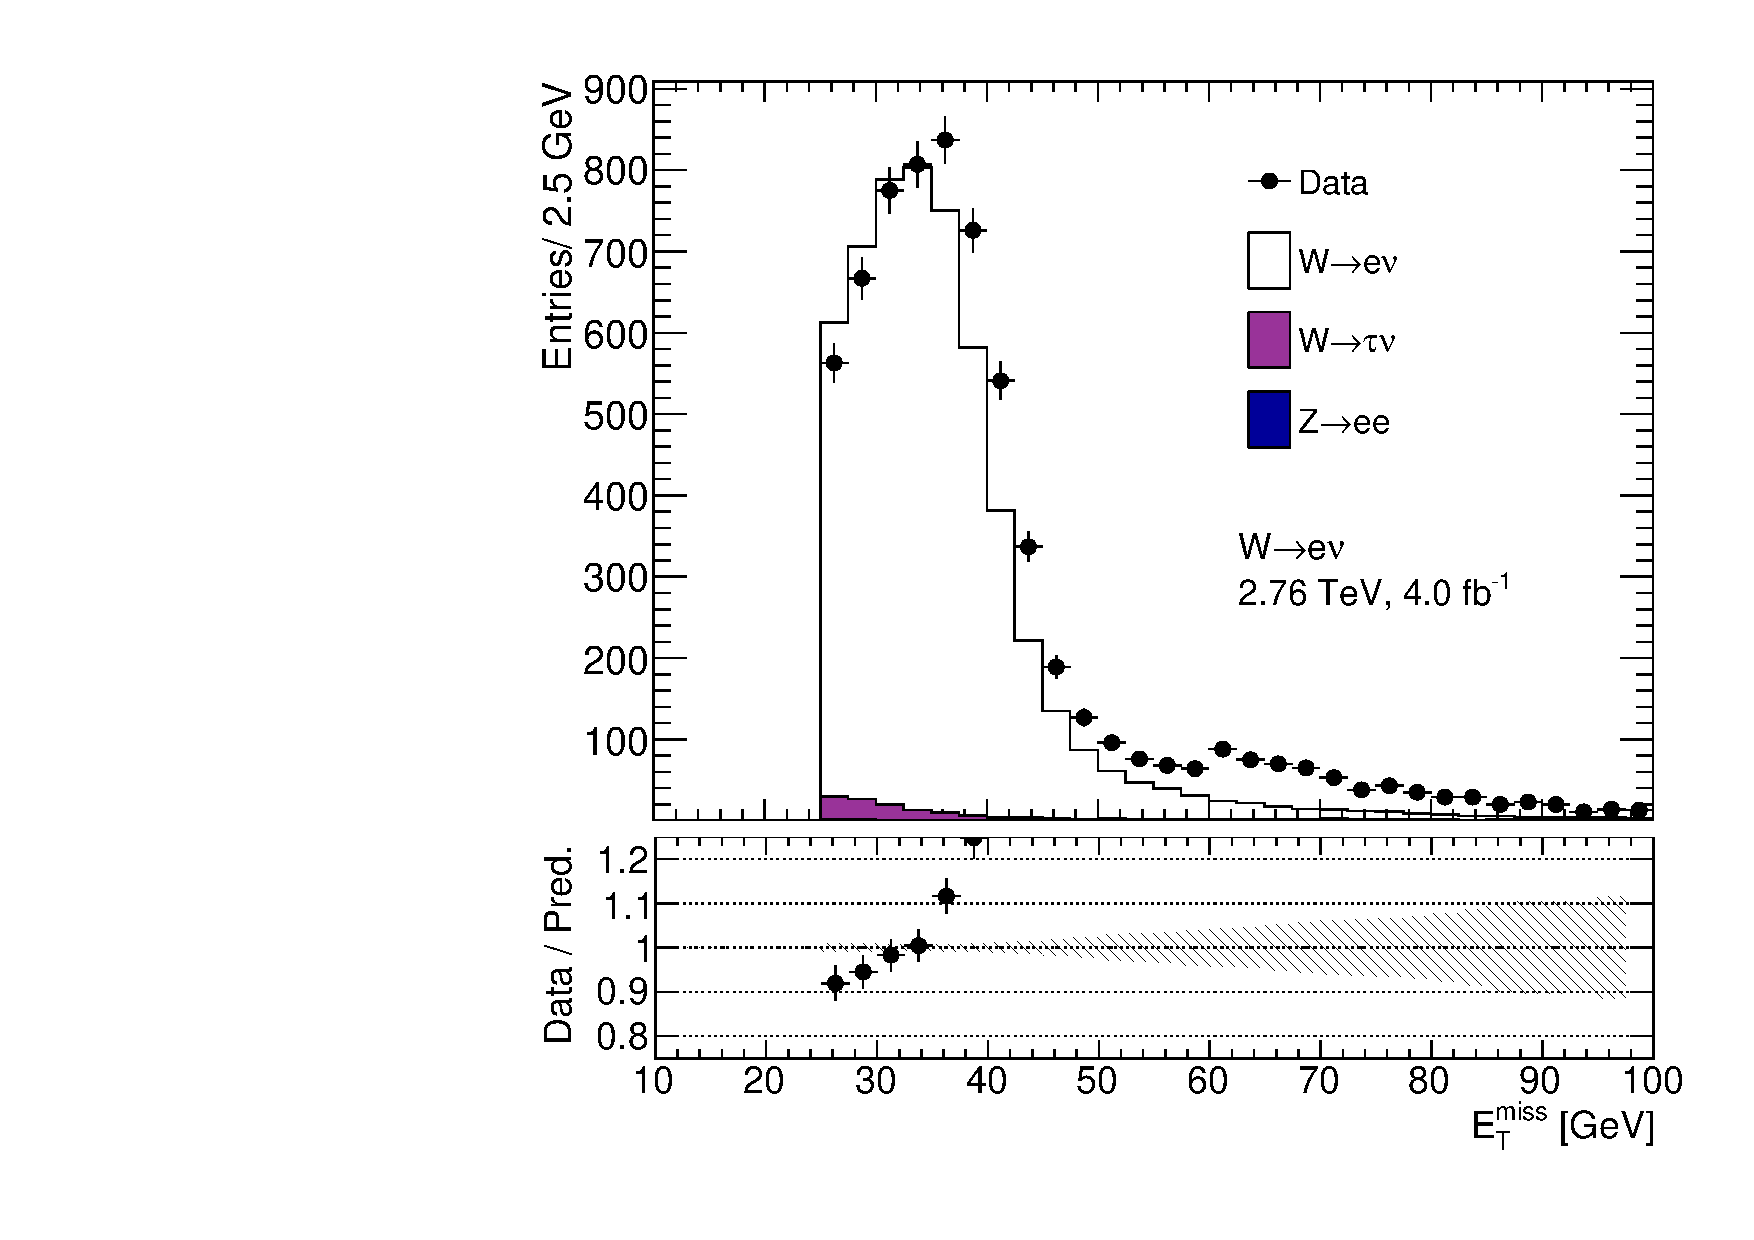
\includegraphics[width=1.\linewidth]{HadronRecoil/WenuRefFinal.pdf} \\ a)}
\end{minipage}
\hfill
\begin{minipage}[h]{0.49\linewidth}
\center{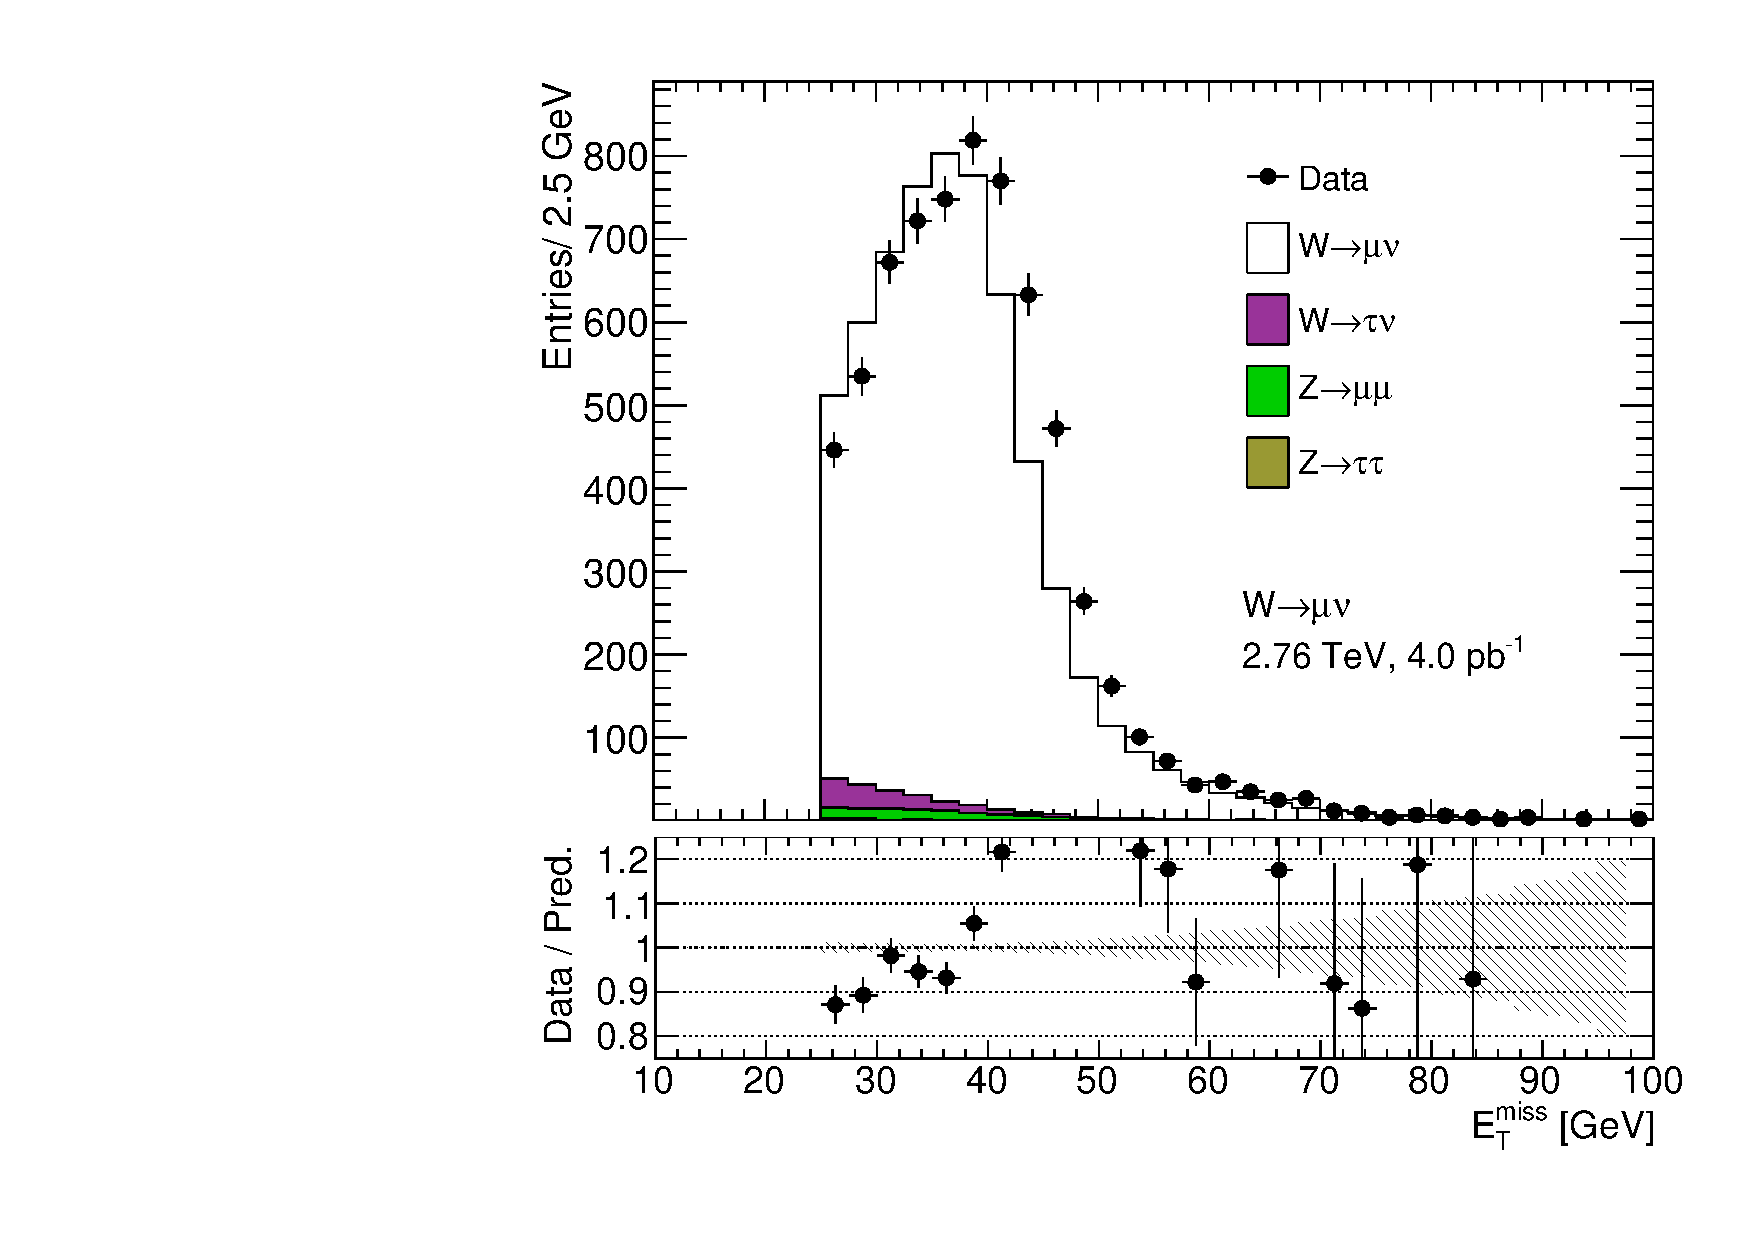
\includegraphics[width=1.\linewidth]{HadronRecoil/WmunuRefFinal.pdf} \\ b)}
\end{minipage}
\caption{Missing transverse energy distribution for a) the \wenu selection and  b) the \wmunu selection from Chap. \ref{chap:EventSelection}. \etmiss  calculated using the standard \atlas algorithm. The expected contributions from all backgrounds are estimated with Monte Carlo simulations, except for QCD background that is not included. All Monte-Carlo corrections from Chap. ~\ref{chap:MCCor} are applied. There are visible discrepancies between data and MC, that cannot be explained by the contribution of QCD background, which is expected mainly in the low \etmiss region (Sec. \ref{sec:QCD}).}
\label{ris:EtMissRefFinal}
\end{figure}

Standard reconstruction of \etmiss at \atlas experiment \cite{Aad2012} uses transverse energy deposits in the calorimeter, energy losses in cryostat and reconstructed muons for a calculation:
\begin{equation}
E_{x(y)}^{miss} = E_{x(y)}^{miss, calo} +  E_{x(y)}^{miss, cryo} +  E_{x(y)}^{miss, muon}.
\end{equation}
Calorimeter term is using information from reconstructed physics objects for calibration of cell responce. The total transverse energy in calorimeter is defined as:
\begin{equation}
E_{x(y)}^{miss} = E_{x(y)}^{miss, e} + E_{x(y)}^{miss, \gamma} + E_{x(y)}^{miss, \tau} + E_{x(y)}^{miss, jets} + E_{x(y)}^{miss,SoftTerm} + E_{x(y)}^{miss, \mu}.
\end{equation}
where each term is calculated as a negative sum of the calibrated reconstructed objects, projected onto the x and y directions. Each jet with energy $P_T$>20 GeV is corrected for a pile-up and a jet energy scale is applied. Soft term is calculated from topoclusters and tracks, that are not assosiated with high-pt objects. To avoid double counting, muon energy loss  in the calorimeter is  subtracted from \etmiss.  The \etmiss muon term is calculated from the momenta of muons measured in a range of pseudorapidity. Since pileup has a significant effect on a \etmiss performance several methods of pileup suppression are used \cite{ATLAS-CONF-2014-019}.

The runs at 2.76 TeV are characterized by a low pileup (mean number of interaction per bunch crossing < 1.0), so the usage of a procedure optimized for high pileup 8 TeV runs may not be optimal. It was examined and figured out, that there are big discrepancies between \etmiss distributions for data and MC simulation, as shown on a Fig. ~\ref{ris:EtMissRefFinal}, where the missing transverse energy for data is compared to signal and background MC predictions. 

The differences are visible in both electron and muon channels and cannot be explained by the (missing on the control plots) contributions from the QCD background, which is expected mainly in the low \etmiss region (see Sec. \ref{sec:QCD}). 



\subsection{Reconstruction of Missing Transverse Energy from hadronic recoil}


\begin{figure}[!tbp]
\begin{center}
\begin{minipage}[h]{0.49\linewidth}
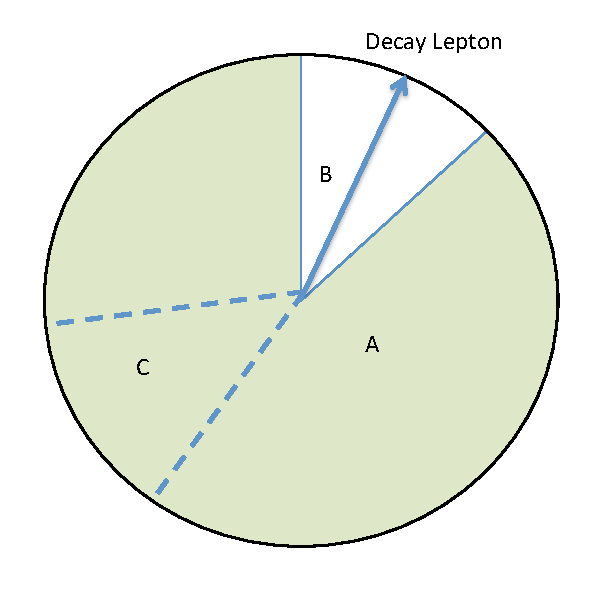
\includegraphics[width=1\textwidth]{HadronRecoil/ReplacementCluster.pdf}
\end{minipage}

\caption{Definition of different zones in the calculation of the cluster-based hadronic recoil. Zone B is excluded from hadron recoil calculation because it contains decay lepton. To describe properly overall acitivity it is replaced by the zone C, rotated in the direction of B. Zone A corresponds to the rest of the calorimeter\cite{HRPlots}.}
\label{ris:subsCone}
\end{center}
\end{figure}

Different way of \etmiss calculation  was developed for W and Z decays by W mass measurements group \cite{HadrRecoilFirst}. This procedure based on the requirement of balance in transverse momentum of a W-boson and the initial (quark-gluon) state radiation:
\begin{equation}
\vec{P}_{T}^{W} = \vec{P}_T^l+\vec{P}_T^{\nu}= \sum{\vec{P}_{T}^{ISRquarks,gluon}}, 
\end{equation}
where $\sum{\vec{P}_{T}^{ISRquarks,gluon}}$ is a transverse momentum of partons from initial state radiation, also called hadronic recoil (HR), $\vec{P}_T^l$ and $\vec{P}_T^{\nu}$ are the transverse momentum of lepton and neutrino respectively. Therefore, \etmiss can be determined as:
\begin{equation}
E_{T}^{miss} = - P_T^{\nu} =  - HR + \ptl
\end{equation} 

This procedure assumes, that recoil arises from one single leading jet, and the rest  is coming from a soft hadronic activity. The hadronic recoil is computed as a vector sum of calorimeter clusters:
\begin{equation}
HR= \sum_{i=0}^{N_{topo}}\vec{p}_T^{topo}
\end{equation}
while a scalar sum of all transverse energy corresponds to the hadronic activity in the event:
\begin{equation}\label{eq:sumet}
\sum E_T =\sum_{i=0}^{N_{topo}} E_T^{topo}
\end{equation}
To avoid double counting of lepton energy losses in the calorimeter, the clusters inside a cone with radius $dR$ = 0.2 around the lepton direction are excluded from this calculation.To compensate for the subtracted soft activity from the cone, a replacement cone is added (Fig. \ref{ris:subsCone}). This cone is defined as a cone at the same pesudorapidity, but a different $\phi$. It should be far from any other lepton and hadron recoil direction. The cone is then rotated to the original lepton direction. This definition does not take into account the jet reconstruction aspects.   

Fig. \ref{ris:HadrRecoilEtMiss} shows the control plots for the distributions of missing transverse energy calculated using the hadronic recoil procedure. In both electron and muon channels the agreement between data and MC simulation is much better than in case of the standard procedure described in a previous chapter. It was desided to use hadronic recoil \etmiss reconstruction method in 2.76 TeV analysis.


\begin{figure}[!tbp]
\begin{minipage}[h]{0.49\linewidth}
\center{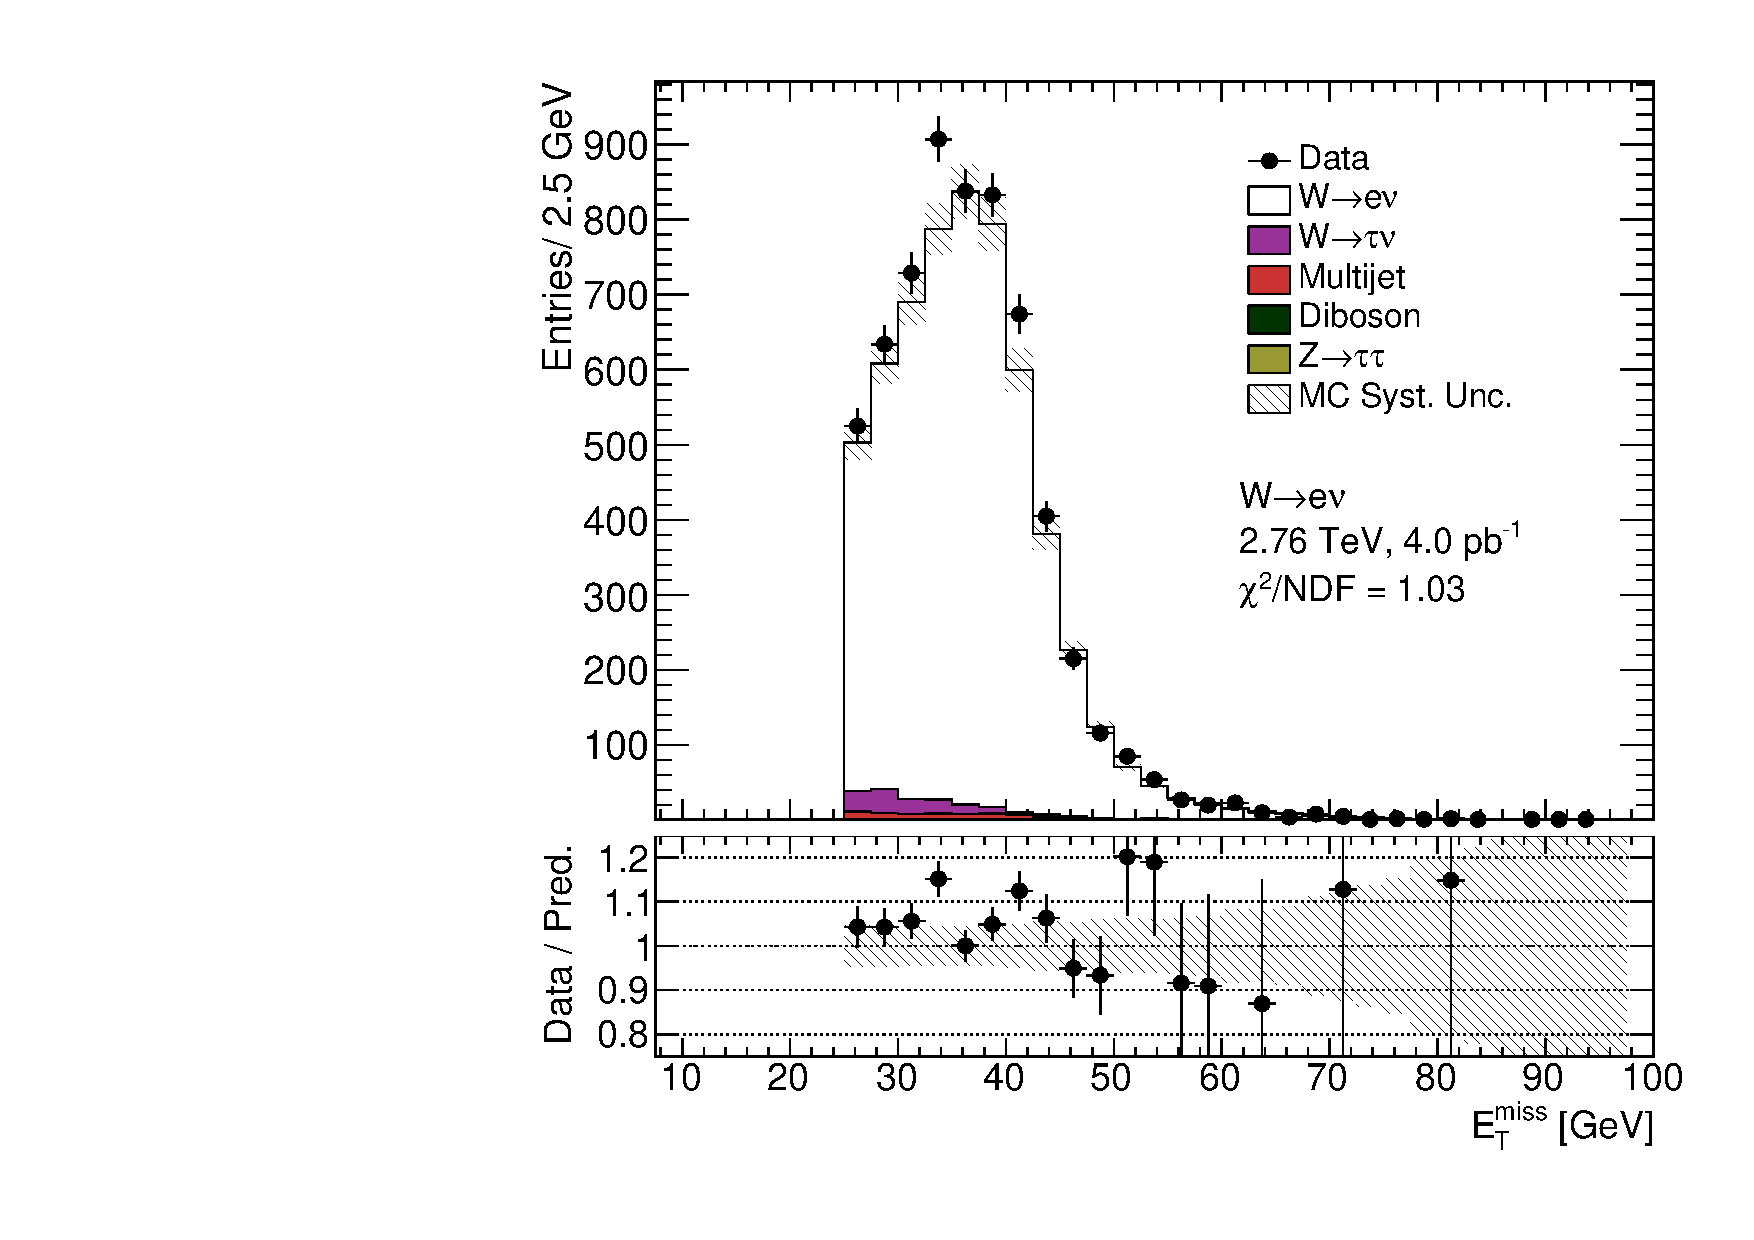
\includegraphics[width=1.\linewidth]{HadronRecoil/W_Boson_etMiss.pdf} \\ a)}
\end{minipage}
\hfill
\begin{minipage}[h]{0.49\linewidth}
\center{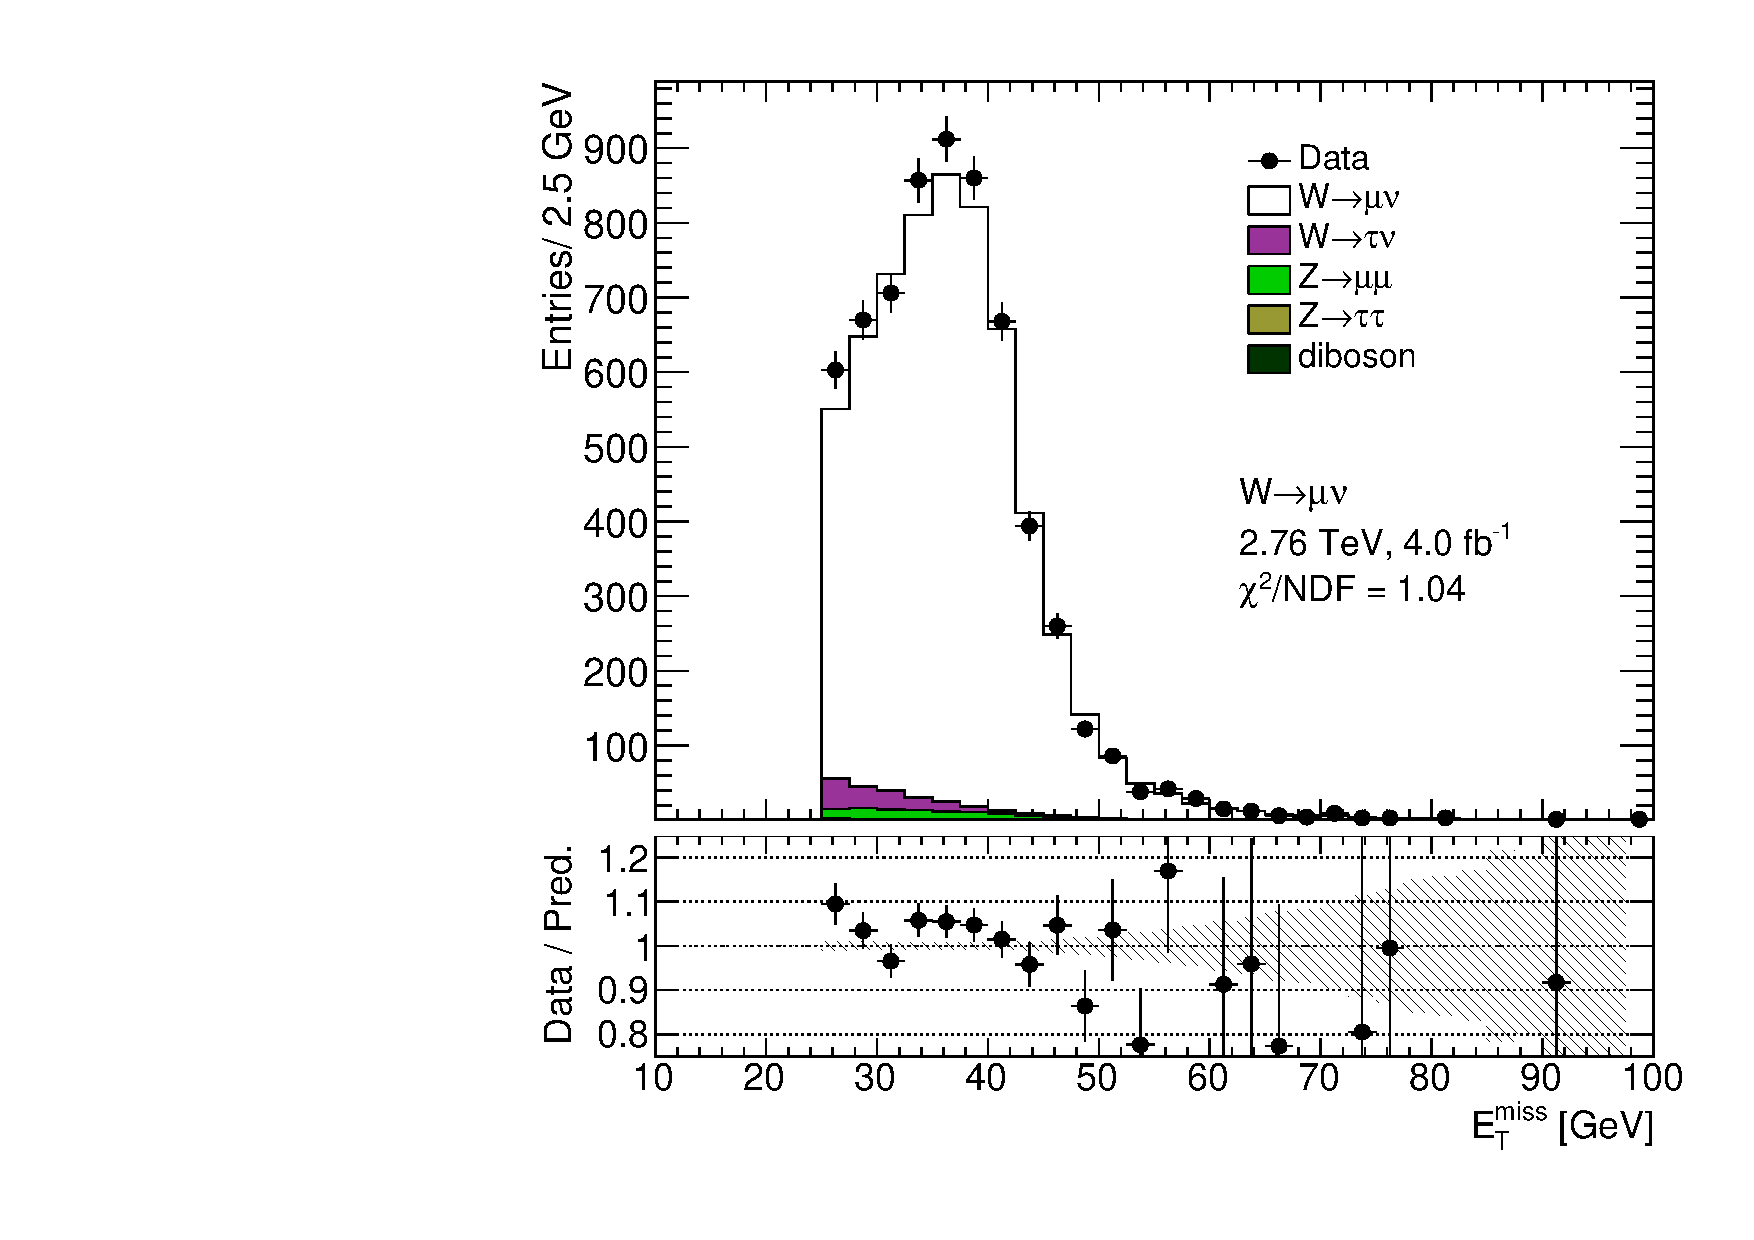
\includegraphics[width=1.\linewidth]{HadronRecoil/Wmu_Boson_etMiss.pdf} \\ b)}
\end{minipage}
\caption{Missing transverse energy distribution for a) the \wenu selection and  b) the \wmunu selection from Chap. \ref{chap:EventSelection}. \etmiss  calculated using the hadronic recoil algorithm. The expected contributions from all backgrounds are estimated with Monte Carlo simulations, except for QCD background that is not included. All Monte-Carlo corrections from Chap. ~\ref{chap:MCCor} are applied.}
\label{ris:HadrRecoilEtMiss}
\end{figure}


